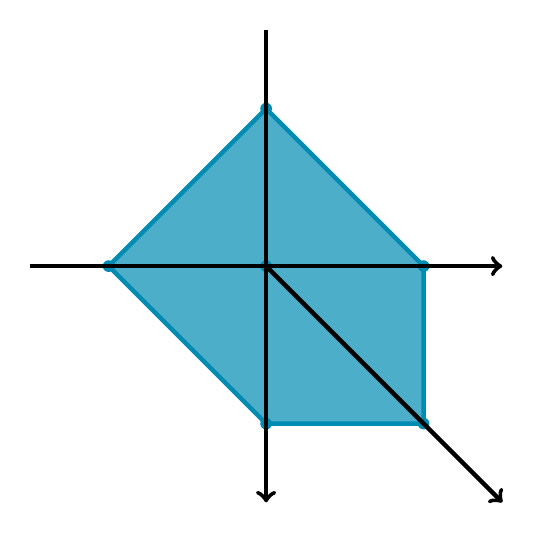
\begin{tikzpicture}

    \def\d{2}
    \def\l{3}
    \def\op{.7}
    \definecolor{blue-ish}{rgb}{0,.55,.7}

    \path (-\l,0) coordinate (3) --++ (\l,0) coordinate (0) --++ (\l,0) coordinate (1);
    \path (0,\l) coordinate (2) --++ (0,-2*\l) coordinate (4) --++ (\l,0) coordinate (5);
    \path (5) --++ (0,2*\l) coordinate (tr) --++ (-2*\l,0) coordinate (tl) --++ (0,-2*\l) coordinate (bl);

    \node [circle, fill, inner sep = 1.5pt, color = blue-ish] (v1) at (\d,0) {};
    \node [circle, fill, inner sep = 1.5pt, color = blue-ish] (v2) at (0,\d) {};
    \node [circle, fill, inner sep = 1.5pt, color = blue-ish] (v3) at (-\d,0) {};
    \node [circle, fill, inner sep = 1.5pt, color = blue-ish] (v4) at (0,-\d) {};
    \node [circle, fill, inner sep = 1.5pt, color = blue-ish] (v5) at (\d,-\d) {};
    \node [circle, fill, inner sep = 1.5pt, color = blue-ish] (v0) at (0,0) {};

    \draw[blue-ish, ultra thick, fill= blue-ish, fill opacity=\op] (v1.center) -- (v2.center) -- (v3.center) -- (v4.center) -- (v5.center) -- cycle;

    \draw[ultra thick, ->] (3) -- (1);
    \draw[ultra thick, ->] (2) -- (4);
    \draw[ultra thick, ->] (0) -- (5);


\end{tikzpicture}

